\documentclass[12pt,a4paper]{report}
\usepackage[utf8]{inputenc}
\usepackage{graphicx}
\usepackage{amsmath}
\usepackage{geometry}
\geometry{a4paper, margin=1in}
\usepackage{mathptmx} % Times New Roman equivalent
\usepackage{titlesec}
\usepackage{caption}
\usepackage{float}
\usepackage{setspace}
\usepackage{fancyhdr}

\titleformat{\chapter}[display]{\normalfont\huge\bfseries}{\chaptertitlename\ \thechapter}{20pt}{\Huge}
\titlespacing*{\chapter}{0pt}{-50pt}{40pt}

\onehalfspacing

\begin{document}

% --- Cover Page ---
\begin{titlepage}
\begin{center}
{\fontsize{28}{34}\selectfont\bfseries Comprehensive Analysis of Field Oriented Control (FOC) for a 3-Phase Induction Motor\par}
\vspace{1.5cm}
{\fontsize{14}{17}\selectfont Project Report Submitted in partial fulfilment of the requirements for the degree of Bachelor of Technology from Maulana Abul Kalam Azad University of Technology, West Bengal (formerly known as West Bengal University of Technology)\par}
\vspace{1.5cm}
{\Large \bfseries By\par}
\vspace{0.5cm}
{\fontsize{18}{22}\selectfont\bfseries
SURJA MONDAL (Roll No. 34901622011)\\
JOYDIP KARMAKAR (Roll No. 34901622014)\\
ANGSU PRIYA ROY (Roll No. 34901622020)\\
HIRAK SINHA (Roll No. 34901622042)\\
KESHAB SARKAR (Roll No. 34901622044)\par}
\vspace{1.5cm}
{\fontsize{16}{19}\selectfont Under the Guidance of\par}
\vspace{0.5cm}
{\fontsize{16}{19}\selectfont Prof. Deepjyoti Santra\par}
\vfill
{\Large Department of Electrical Engineering\par}
{\Large Cooch Behar Government Engineering College\par}
{\Large Cooch Behar, West Bengal\par}
{\Large 2026\par}
\end{center}
\end{titlepage}

% --- Certificate of Recommendation ---
\newpage
\begin{center}
{\Large \bfseries Certificate of Recommendation\par}
\end{center}
\vspace{1cm}
It is hereby recommended to consider the project report entitled ``Comprehensive Analysis of Field Oriented Control (FOC) for a 3-Phase Induction Motor'' submitted by SURJA MONDAL (Roll No. 34901622011), JOYDIP KARMAKAR (Roll No. 34901622014), ANGSU PRIYA ROY (Roll No. 34901622020), HIRAK SINHA (Roll No. 34901622042), and KESHAB SARKAR (Roll No. 34901622044) for partial fulfillment of the requirements for the award of the degree of Bachelor of Technology in Electrical Engineering from Maulana Abul Kalam Azad University of Technology (formerly known as West Bengal University of Technology).
\vspace{3cm}

\noindent
\begin{tabular}{@{}p{8cm}p{8cm}@{}}
------------------------------ & ------------------------------- \\
Prof. Deepjyoti Santra & Prof. Atanu Maji \\
Project Guide & (Head of Electrical Engg. Department)
\end{tabular}

% --- Certificate of Approval ---
\newpage
\begin{center}
{\Large \bfseries Certificate of Approval\par}
\end{center}
\vspace{1cm}
It is hereby approved that the project report entitled ``Comprehensive Analysis of Field Oriented Control (FOC) for a 3-Phase Induction Motor'' submitted by SURJA MONDAL (Roll No. 34901622011), JOYDIP KARMAKAR (Roll No. 34901622014), ANGSU PRIYA ROY (Roll No. 34901622020), HIRAK SINHA (Roll No. 34901622042), and KESHAB SARKAR (Roll No. 34901622044) for partial fulfilment of the requirements for the award of the degree of Bachelor of Technology in Electrical Engineering from Maulana Abul Kalam Azad University of Technology (formerly known as West Bengal University of Technology).
\vspace{3cm}

\noindent Board of Examiners
\vspace{1.5cm}

\noindent --------------------------- \\
\vspace{1cm}

\noindent --------------------------- \\
\vspace{1cm}

\noindent ---------------------------

% --- Acknowledgement ---
\newpage
\begin{center}
{\Large \bfseries Acknowledgement\par}
\end{center}
\vspace{1cm}
We would like to express our profound gratitude to our project guide, Prof. Deepjyoti Santra, for his valuable guidance, continuous support, and encouragement throughout the course of this project. We are also deeply thankful to Prof. Atanu Maji, Head of the Electrical Engineering Department, for providing us with the necessary facilities and a conducive environment to carry out this work.

We also extend our heartfelt thanks to the faculty and staff of Cooch Behar Government Engineering College for their continuous assistance and cooperation.

\vspace{2cm}
\begin{flushright}
SURJA MONDAL (34901622011)\\
JOYDIP KARMAKAR (34901622014)\\
ANGSU PRIYA ROY (34901622020)\\
HIRAK SINHA (34901622042)\\
KESHAB SARKAR (34901622044)
\end{flushright}

% --- TOC, LOF, LOT ---
\newpage
\tableofcontents
\newpage
\listoffigures
\newpage
\listoftables

% --- Abstract ---
\newpage
\begin{center}
{\Large \bfseries Abstract\par}
\end{center}
\vspace{1cm}
This report provides a comprehensive, component-level technical analysis of the Simulink model \texttt{VECTOR\_CONTROL\_FOC\_OF\_IM.slx}, which implements an Indirect Field Oriented Control (IFOC) architecture for a 50 HP Squirrel-Cage Induction Motor. Intended as an advanced instructional document for graduate-level electrical machines and drives coursework, this report systematically deconstructs the theoretical and practical frameworks embedded within the simulation. It begins by establishing the plant's equivalent circuit parameters and dynamic modelling, supplemented with detailed mathematical calculations demonstrating the derivation of time constants, inductances, and torque parameters. 

The analysis then explores the critical coordinate transformations (Forward and Reverse Clarke and Park) required to map stationary three-phase variables into a synchronously rotating $d-q$ reference frame. By examining the system's decoupling equations, the report demonstrates how IFOC achieves independent, high-performance regulation of rotor flux and electromagnetic torque effectively mirroring the transient dynamics of a separately excited DC machine. Furthermore, the document evaluates the discrete-time closed-loop control strategy, detailing the tuning parameters and anti-windup mechanisms of the cascaded Proportional-Integral (PI) controllers used in the outer speed and inner current loops. Finally, the report dissects the Space Vector Pulse Width Modulation (SVPWM) synthesis used to drive the three-phase inverter, highlighting its advantages in optimising DC bus utilisation and minimising total harmonic distortion (THD).

% --- Chapters ---
\chapter{INTRODUCTION}
\section{Introduction}
Traditionally, the control of induction machines was dominated by scalar methods, such as constant Volts-per-Hertz ($V/f$) control. While adequate for basic steady-state operations, scalar control governs only the magnitude and frequency of the applied voltage and currents, fundamentally ignoring the spatial orientation of the electromagnetic fields. Consequently, scalar methods suffer from sluggish transient responses, cross-coupling effects, and an inability to independently regulate torque and flux during dynamic state changes.

Field Oriented Control (FOC), also known as Vector Control, represents a revolutionary paradigm shift in AC machine drives, overcoming the limitations of scalar control. The fundamental objective of FOC is to emulate the highly desirable, decoupled control dynamics of a separately excited DC motor. In a traditional DC machine, the field flux and the armature flux are maintained in a strict state of spatial orthogonality by the mechanical commutator. This decoupling allows the field current and armature current to be manipulated independently to control magnetic flux and electromagnetic torque, yielding instantaneous dynamic response.

\section{Review of Previous Works (Literature Review)}
Historically, Field Oriented Control was developed to address the non-linear, multi-variable control challenge inherent in three-phase Induction Motors. Direct Field Oriented Control (DFOC) utilised air-gap sensors or observers to measure flux, which often proved fragile or noisy. Indirect Field Oriented Control (IFOC), on the other hand, mathematically synthesises the flux angle using feedforward slip calculations, greatly improving the robustness and dynamic performance of the drive system.

\section{Objective and Motivation}
The objective of this project is to model, simulate, and mathematically validate a complete Indirect FOC architecture for a 50 HP Induction Motor using MATLAB/Simulink. The motivation is to thoroughly understand the decoupling of flux-producing and torque-producing current components, observe the dynamic performance under varying speed and torque conditions, and implement advanced Space Vector PWM (SVPWM) to optimize inverter switching.

\section{Scope of Present Work}
This report comprehensively covers the induction motor's mathematical modelling, FOC component derivations (Clarke and Park transforms), dynamic decoupling, and SVPWM logic. Extensive simulations are presented, showcasing the system's performance metrics through scope analyses of torque transients, speed tracking, current waveforms, and dwell times.

\begin{figure}[H]
    \centering
    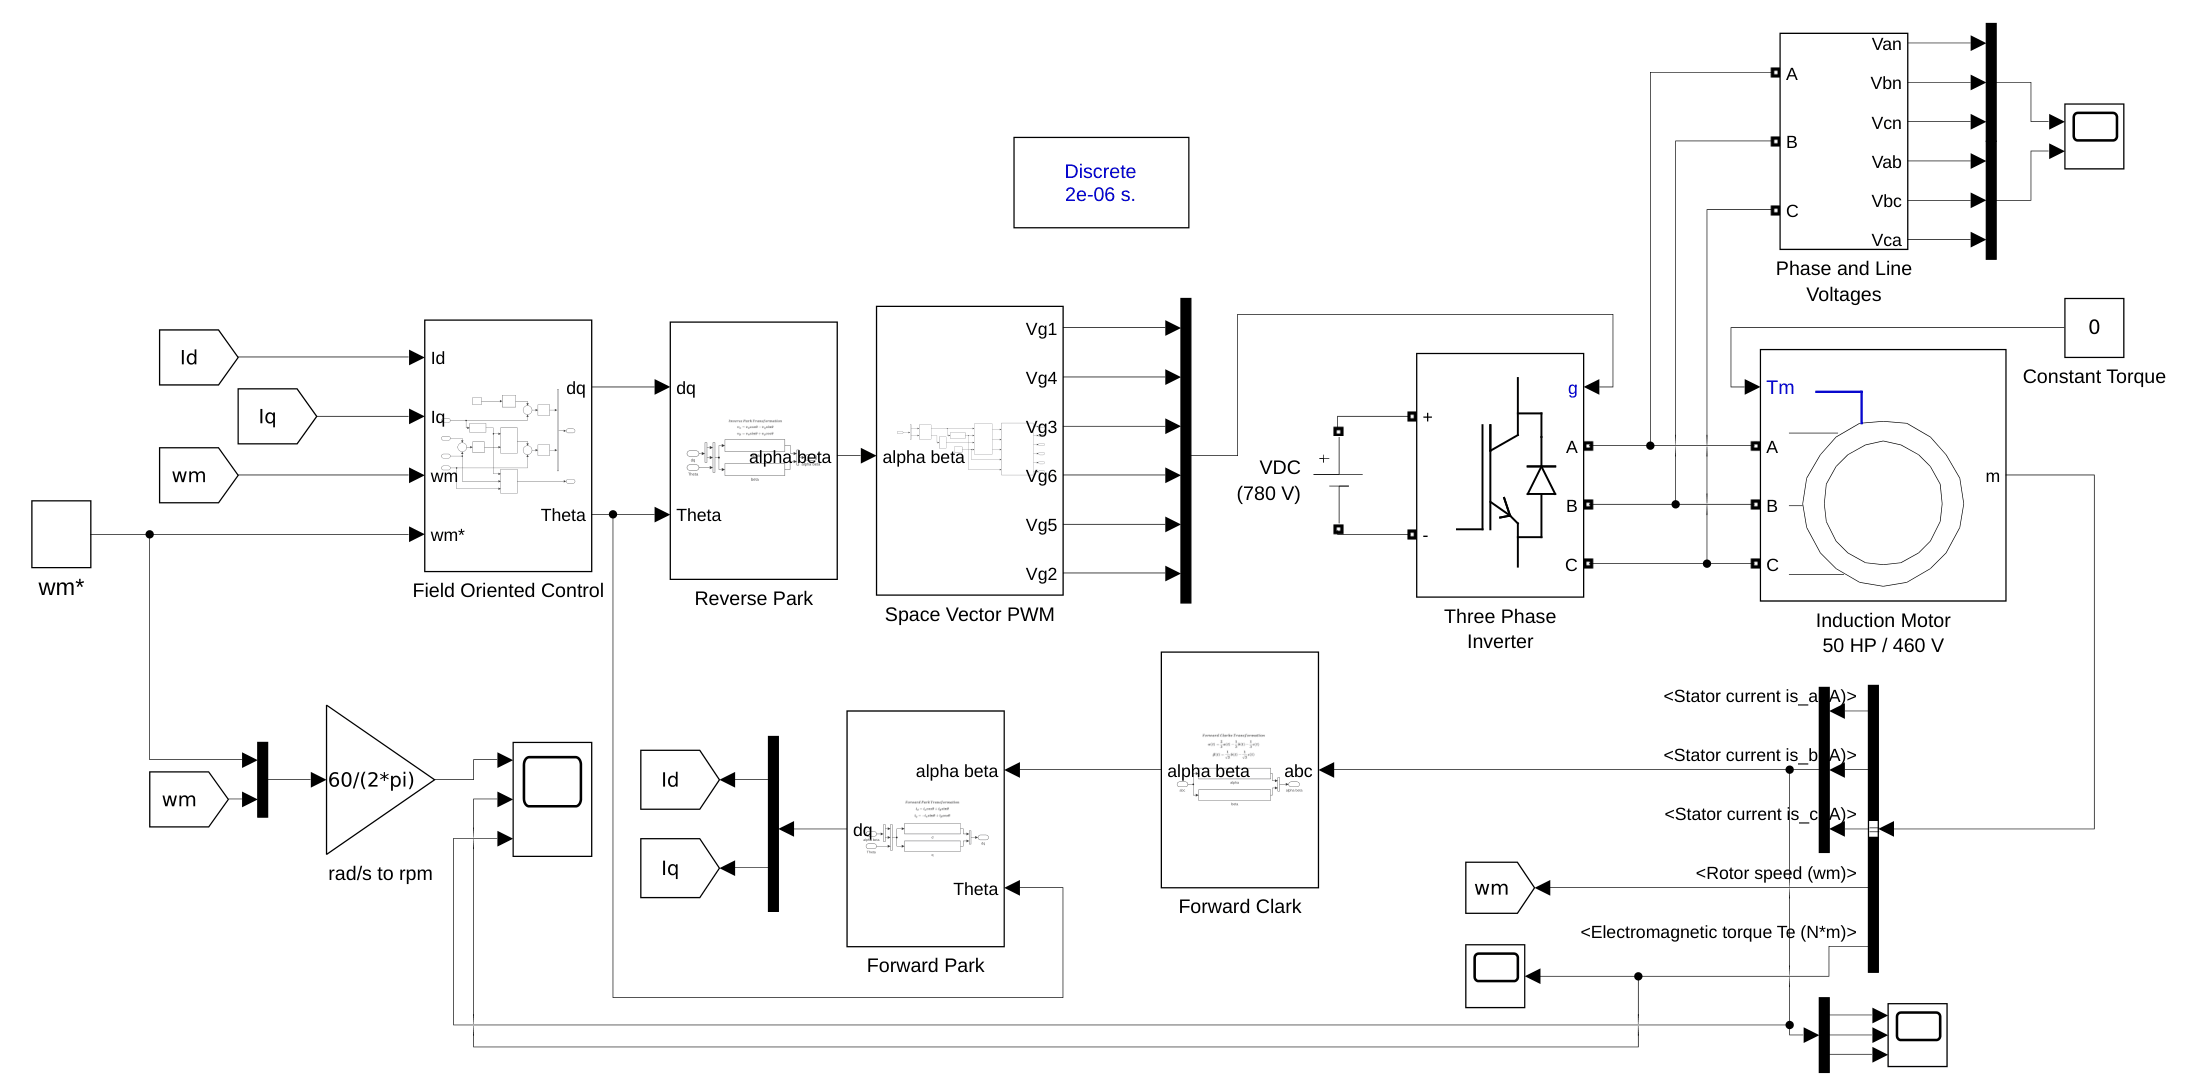
\includegraphics[width=0.9\textwidth]{VECTOR_CONTROL_FOC_OF_IM-01.png}
    \caption{Top-Level Simulink Model Architecture of the FOC for Induction Motor}
\end{figure}


\chapter{Induction Motor Plant Parameters and Dynamic Modelling}
\section{Plant Parameters and Equivalent Circuit}
The electromechanical plant governed by this control architecture is a three-phase Squirrel-Cage Induction Motor (SCIM). The squirrel-cage design presents a unique challenge: the rotor currents and rotor flux linkages are physically inaccessible and cannot be directly measured. Consequently, the control strategy relies entirely on an accurate mathematical model of the machine, dictated by its equivalent circuit parameters.

Based on the model's initialization routines, the motor is defined by the following ratings:
\begin{table}[H]
\centering
\caption{Squirrel-Cage Induction Motor Nominal Ratings and Equivalent Circuit Parameters}
\begin{tabular}{|p{3cm}|p{8cm}|p{4cm}|}
\hline
\textbf{Symbol} & \textbf{Parameter Description} & \textbf{Value} \\ \hline
$S$ & Nominal Power & 50 HP (37.3 kW) \\ \hline
$V_{s}$ & Stator Line-to-Line Voltage & 460 V \\ \hline
$f$ & Nominal Frequency & 50 Hz \\ \hline
$P$ & Number of Poles & 4 (2 Pole Pairs) \\ \hline
$N_{s}$ & Synchronous Speed & 1500 RPM \\ \hline
$R_{s}$ & Stator Resistance & 0.087 $\Omega$ \\ \hline
$R_{r}$ & Rotor Resistance (Referred to Stator) & 0.228 $\Omega$ \\ \hline
$L_{ls}$ & Stator Leakage Inductance & 0.1 mH \\ \hline
$L_{lr}$ & Rotor Leakage Inductance (Referred) & 0.8 mH \\ \hline
$L_{m}$ & Magnetizing Inductance & 34.7 mH \\ \hline
$J$ & Moment of Inertia & 0.662 kg.m$^2$ \\ \hline
$F$ & Viscous Friction Coefficient & 0.1 Nms/rad \\ \hline
\end{tabular}
\end{table}

\section{Significance of Electrical Parameters in FOC}
From the values provided, the lumped self-inductances of the stator ($L_s$) and rotor ($L_r$) are calculated as follows:
\begin{align}
L_{s} &= L_{ls} + L_{m} = 0.1 \text{ mH} + 34.7 \text{ mH} = 34.8 \text{ mH} = 0.0348 \text{ H} \\
L_{r} &= L_{lr} + L_{m} = 0.8 \text{ mH} + 34.7 \text{ mH} = 35.5 \text{ mH} = 0.0355 \text{ H}
\end{align}

A critical derived parameter in Indirect Field Oriented Control is the rotor time constant ($\tau_r$):
\begin{equation}
\tau_{r} = \frac{L_{r}}{R_{r}} = \frac{35.5 \times 10^{-3}}{0.228} \approx 0.155701 \text{ seconds}
\end{equation}
The accuracy of $\tau_{r}$ is absolutely paramount for feedforward slip-calculation. If the value of $R_{r}$ deviates during operation (e.g., thermal heating), $\tau_{r}$ changes, leading to a phenomenon known as detuning, which causes spatial misalignment between the expected and actual $d-q$ axes.

The machine's total leakage factor ($\sigma$), which dictates the required bandwidth of the inner PI current controllers, is calculated as:
\begin{equation}
\sigma = 1 - \frac{L_{m}^2}{L_{s}L_{r}} = 1 - \frac{(0.0347)^2}{(0.0348 \times 0.0355)} = 1 - \frac{0.00120409}{0.0012354} = 1 - 0.97465 = 0.02535
\end{equation}
This small value ($\sigma \ll 1$) indicates a highly coupled magnetic circuit, necessitating fast-acting current loops.

\section{Mechanical Dynamics and Speed Loop Tuning}
The mechanical equation of motion that dictates the rotor's dynamic trajectory is governed by:
\begin{equation}
T_{e} - T_{L} = J\frac{d\omega_{m}}{dt} + F\omega_{m}
\end{equation}
Substituting the mechanical parameters of the 50 HP motor ($J=0.662, F=0.1$):
\begin{equation}
T_{e} - T_{L} = 0.662\frac{d\omega_{m}}{dt} + 0.1\cdot\omega_{m}
\end{equation}
Taking the Laplace transform yields the mechanical transfer function:
\begin{equation}
\frac{\omega_{m}(s)}{T_{e}(s)} = \frac{1}{0.662s + 0.1}
\end{equation}

\begin{figure}[H]
    \centering
    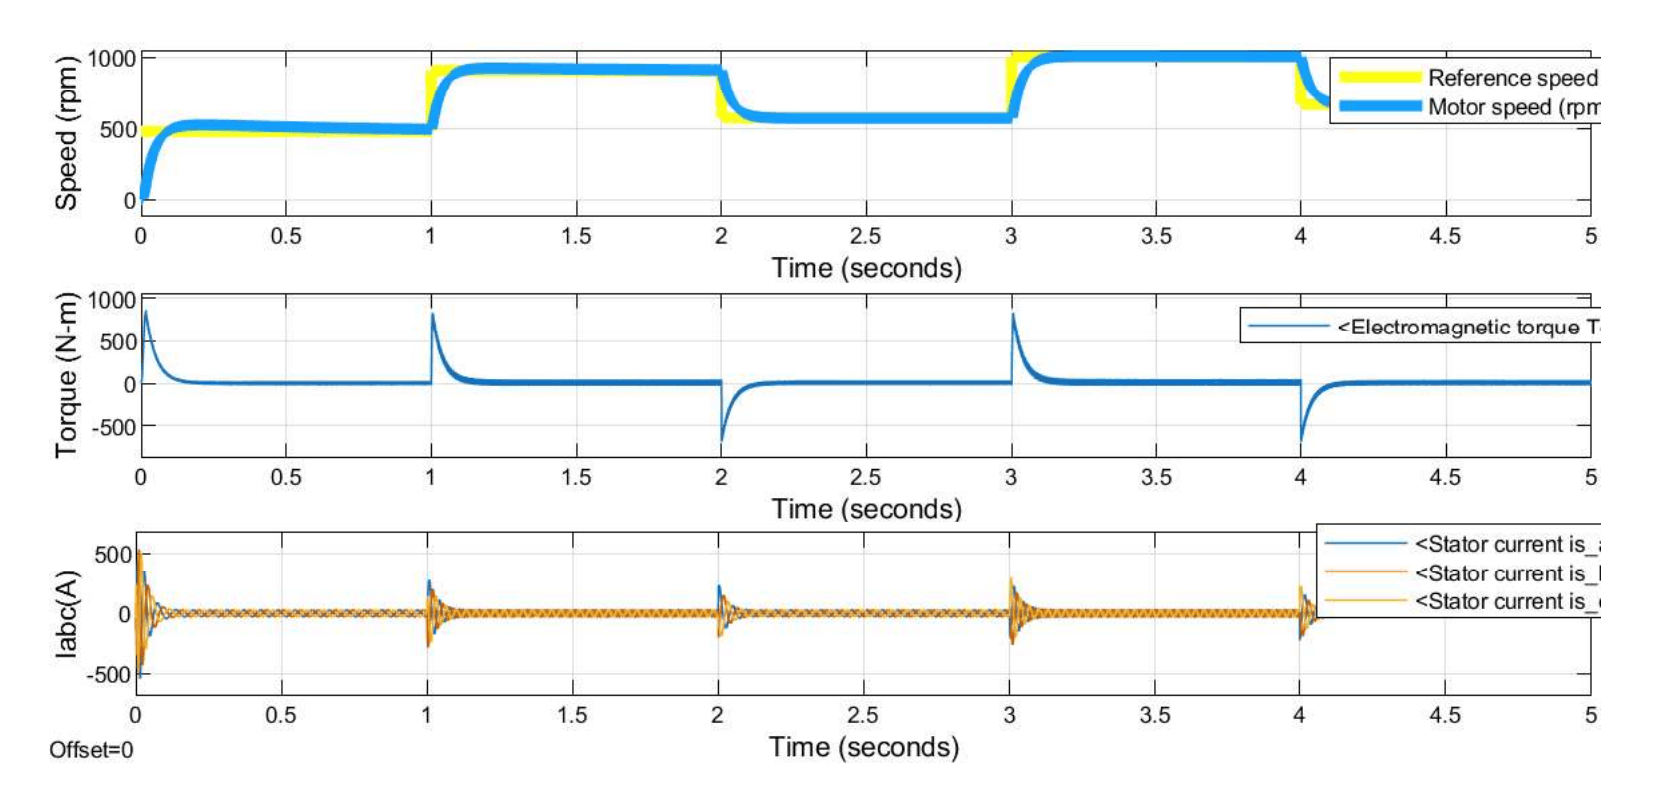
\includegraphics[width=0.9\textwidth]{7.png}
    \caption{Scope Output: Performance of the Speed Control Loop Tracking Step Changes}
\end{figure}
\begin{figure}[H]
    \centering
    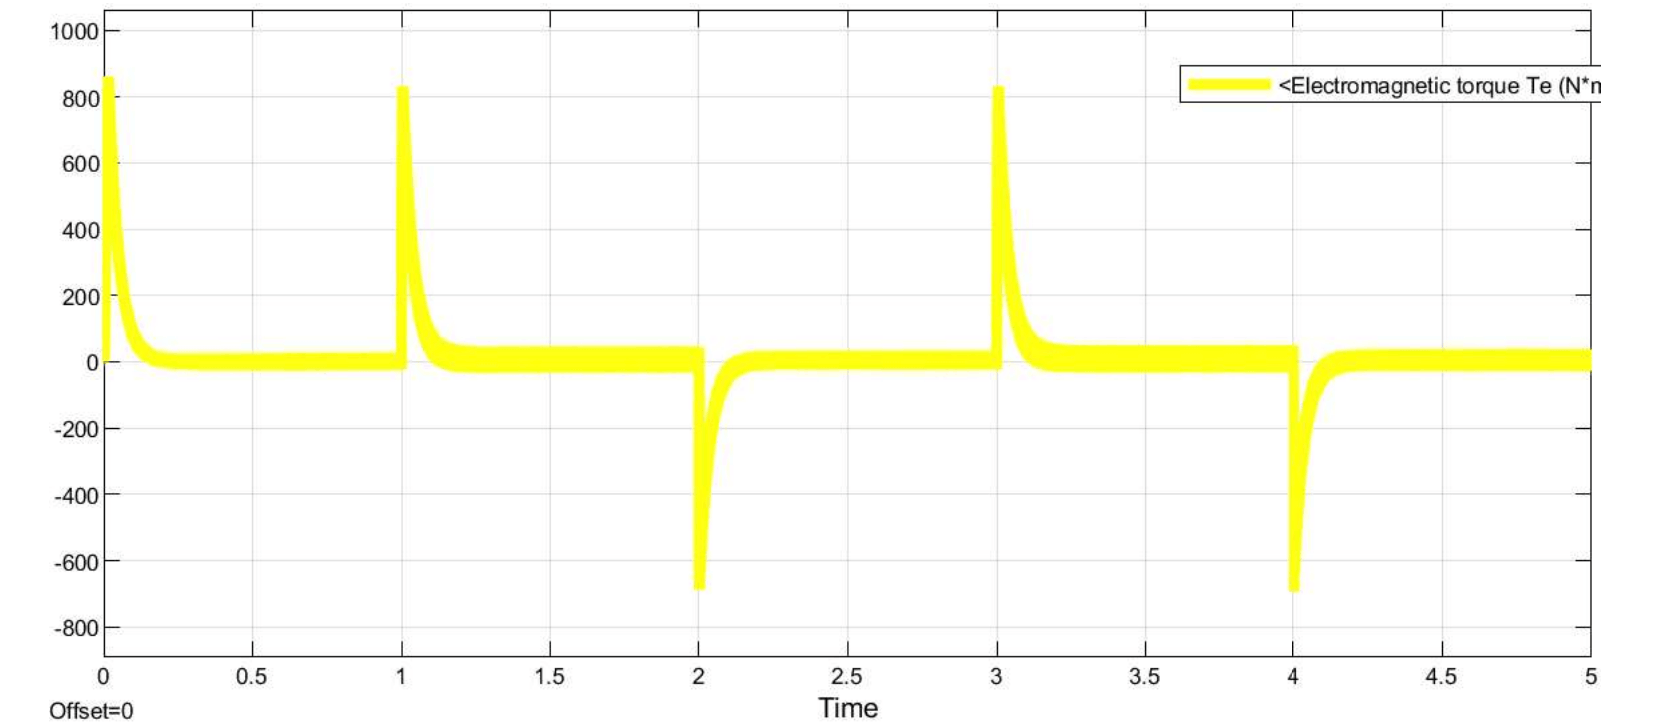
\includegraphics[width=0.9\textwidth]{1.png}
    \caption{Scope Output: Transient and Steady-State Electromechanical Torque ($T_e$)}
\end{figure}

\chapter{Control System Architecture and Discrete-Time Execution}
\section{Coordinate Transformations}
To control the multi-phase AC induction machine as effectively as a DC motor, FOC relies on resolving the three-phase, time-variant stator currents into a synchronously rotating reference frame ($d-q$).

\subsection{Forward Clarke Transform (Stationary $3 \rightarrow 2$ Projection)}
The Clarke transform maps the three-phase currents ($i_a, i_b, i_c$) into two-phase orthogonal stationary coordinates ($i_\alpha, i_\beta$):
\begin{equation}
\begin{bmatrix} i_{\alpha} \\ i_{\beta} \end{bmatrix} = \frac{2}{3} \begin{bmatrix} 1 & -\frac{1}{2} & -\frac{1}{2} \\ 0 & \frac{\sqrt{3}}{2} & -\frac{\sqrt{3}}{2} \end{bmatrix} \begin{bmatrix} i_{a} \\ i_{b} \\ i_{c} \end{bmatrix}
\end{equation}
For example, assuming balanced stator currents with a peak of 100 A (e.g., $i_a=100A, i_b=-50A, i_c=-50A$ at $\omega t = 0$):
\begin{align}
i_{\alpha} &= \frac{2}{3}(1(100) - 0.5(-50) - 0.5(-50)) = \frac{2}{3}(100 + 25 + 25) = 100 \text{A} \\
i_{\beta} &= \frac{2}{3}(0(100) + 0.866(-50) - 0.866(-50)) = 0 \text{A}
\end{align}

\begin{figure}[H]
    \centering
    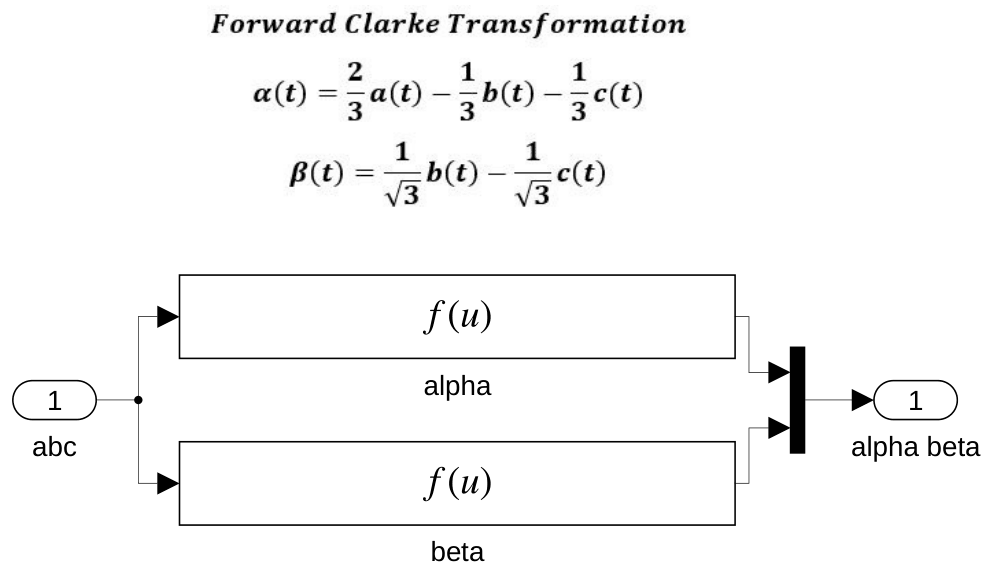
\includegraphics[width=0.8\textwidth]{VECTOR_CONTROL_FOC_OF_IM-06.png}
    \caption{Simulink Subsystem: Forward Clarke Transform}
\end{figure}

\subsection{Forward Park Transform (Stationary $\alpha-\beta$ to Rotating $d-q$)}
The Park transform locks the observer's perspective to the spinning magnetic field:
\begin{equation}
\begin{bmatrix} i_{d} \\ i_{q} \end{bmatrix} = \begin{bmatrix} \cos\theta_{e} & \sin\theta_{e} \\ -\sin\theta_{e} & \cos\theta_{e} \end{bmatrix} \begin{bmatrix} i_{\alpha} \\ i_{\beta} \end{bmatrix}
\end{equation}

\begin{figure}[H]
    \centering
    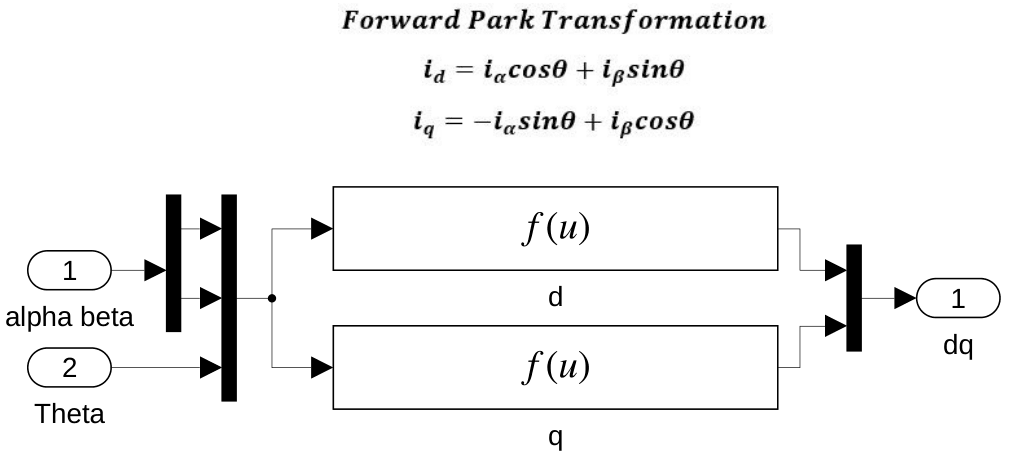
\includegraphics[width=0.8\textwidth]{VECTOR_CONTROL_FOC_OF_IM-07.png}
    \caption{Simulink Subsystem: Forward Park Transform}
\end{figure}
\begin{figure}[H]
    \centering
    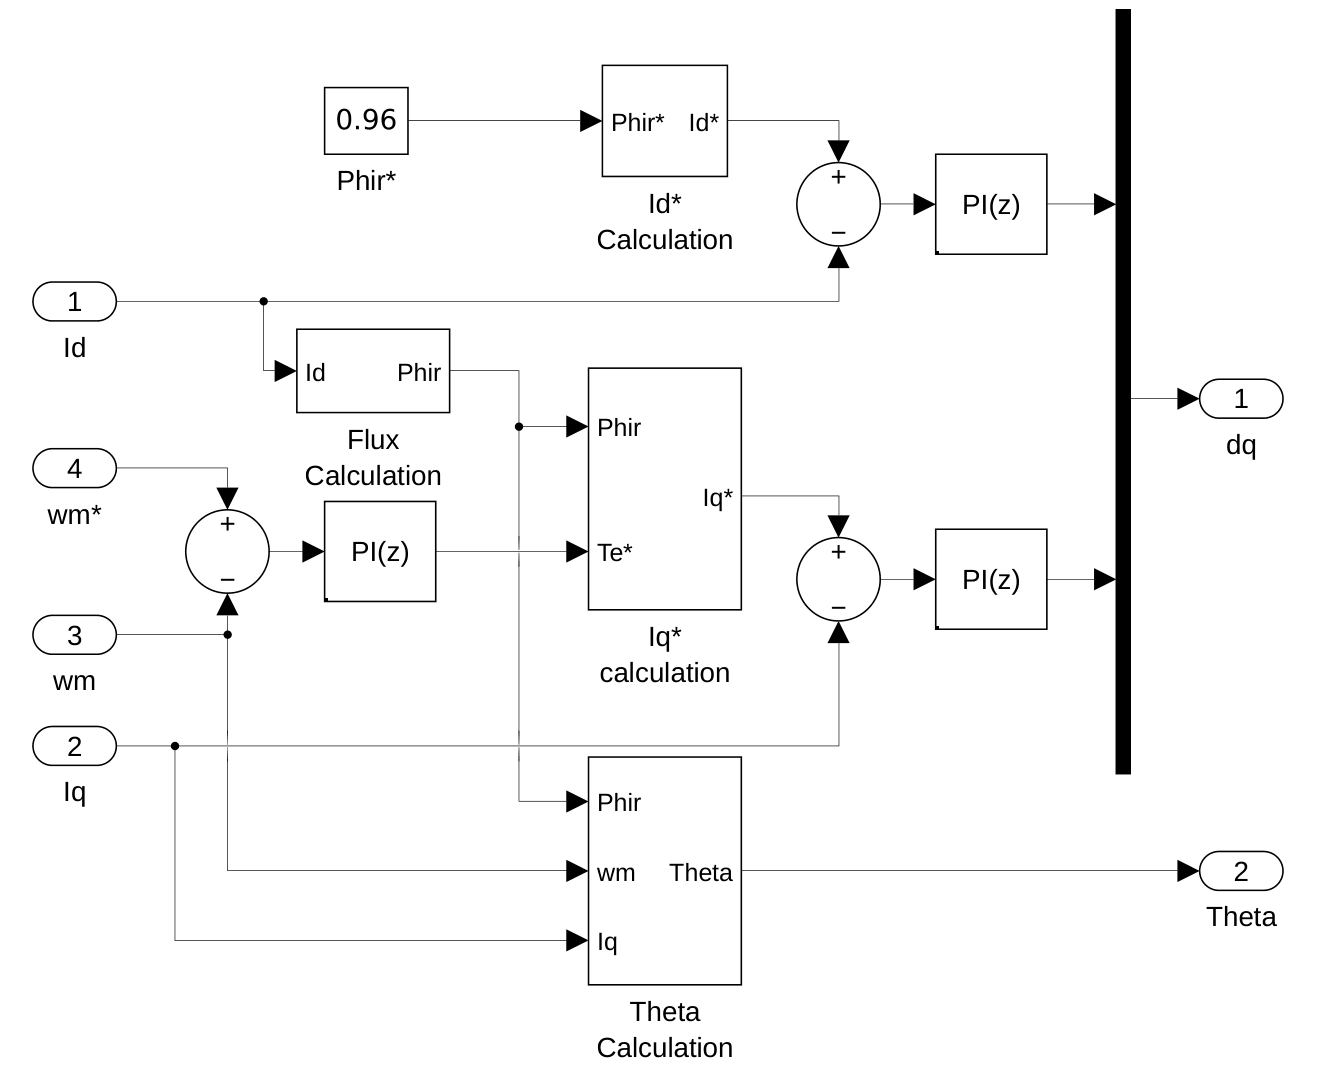
\includegraphics[width=0.9\textwidth]{VECTOR_CONTROL_FOC_OF_IM-02.png}
    \caption{Detailed Implementation of FOC Control Loops}
\end{figure}

\subsection{Reverse Park Transform}
Once the PI controllers have generated the decoupling voltage commands ($v_d^*, v_q^*$), they must be de-rotated into the stationary frame for the inverter:
\begin{equation}
\begin{bmatrix} v_{\alpha}^* \\ v_{\beta}^* \end{bmatrix} = \begin{bmatrix} \cos\theta_{e} & -\sin\theta_{e} \\ \sin\theta_{e} & \cos\theta_{e} \end{bmatrix} \begin{bmatrix} v_{d}^* \\ v_{q}^* \end{bmatrix}
\end{equation}

\begin{figure}[H]
    \centering
    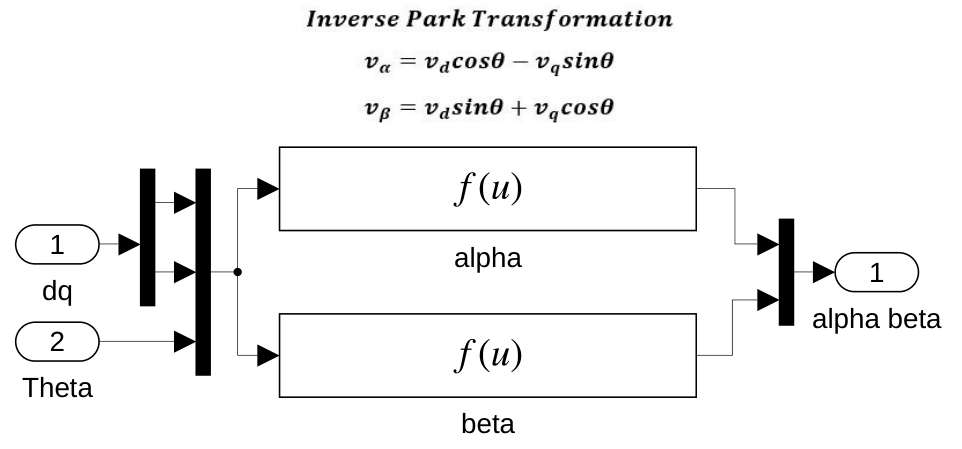
\includegraphics[width=0.8\textwidth]{VECTOR_CONTROL_FOC_OF_IM-09.png}
    \caption{Simulink Subsystem: Reverse Park Transform}
\end{figure}

\section{Flux and Torque Decoupling Equations}
\subsection{Direct-Axis Current Reference ($i_{ds}^*$)}
The transient behaviour of the rotor flux linkage $\psi_{r}$ is governed by:
\begin{equation}
\tau_{r}\frac{d\psi_{r}}{dt} + \psi_{r} = L_{m}i_{ds}
\end{equation}
Substituting our derived values ($\tau_r = 0.1557$, $L_m = 0.0347$):
\begin{equation}
0.1557\frac{d\psi_{r}}{dt} + \psi_{r} = 0.0347 \cdot i_{ds}
\end{equation}
In steady-state IFOC, the derivative term is zero. Thus, for a desired nominal flux $\psi_{r}^* = 0.96$ Wb:
\begin{equation}
i_{ds}^* = \frac{\psi_{r}^*}{L_{m}} = \frac{0.96}{0.0347} = 27.6657 \text{ A}
\end{equation}
\begin{figure}[H]
    \centering
    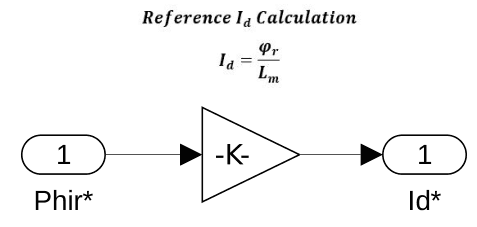
\includegraphics[width=0.7\textwidth]{VECTOR_CONTROL_FOC_OF_IM-03.png}
    \caption{Simulink Subsystem: $I_{d}^*$ Reference Calculation Block}
\end{figure}

\subsection{Quadrature-Axis Current Reference ($i_{qs}^*$)}
The general expression for the electromagnetic torque is:
\begin{equation}
T_{e} = \frac{3}{2}\left(\frac{P}{2}\right)\frac{L_{m}}{L_{r}}(\psi_{dr}i_{qs} - \psi_{qr}i_{ds})
\end{equation}
By orienting the d-axis exactly with the rotor flux, we enforce $\psi_{qr}=0$ and $\psi_{dr} = \psi_{r}$:
\begin{equation}
T_{e} = \frac{3}{2}\left(\frac{4}{2}\right)\left(\frac{0.0347}{0.0355}\right)(0.96 \cdot i_{qs}) = 2.9324(0.96 \cdot i_{qs}) = 2.8152 \cdot i_{qs} \text{ N}\cdot\text{m}
\end{equation}
Inverting this to solve for the reference current dynamically:
\begin{equation}
i_{qs}^* = \frac{2}{3} \cdot \frac{2}{P} \cdot \frac{L_{lr} + L_{m}}{L_{m}} \cdot \frac{T_{e}^*}{\psi_{r} + 10^{-3}}
\end{equation}
Isolating $i_{qs}^*$ algebraically:
\begin{equation}
i_{qs}^* = \left(\frac{2}{3}\right)\left(\frac{2}{4}\right)\left(\frac{0.0355}{0.0347}\right)\frac{T_{e}^*}{0.96} = (0.3333) \times (1.02305) \times \frac{T_{e}^*}{0.96} = 0.3552 \cdot T_{e}^* \text{ A}
\end{equation}
For a nominal torque of 100 Nm, the control logic demands $35.52$ A of torque-producing current. A small numerical offset ($\epsilon = 10^{-3}$) is utilized to prevent division-by-zero singularities upon motor start-up when initial flux $\psi_{r} = 0$.

\begin{figure}[H]
    \centering
    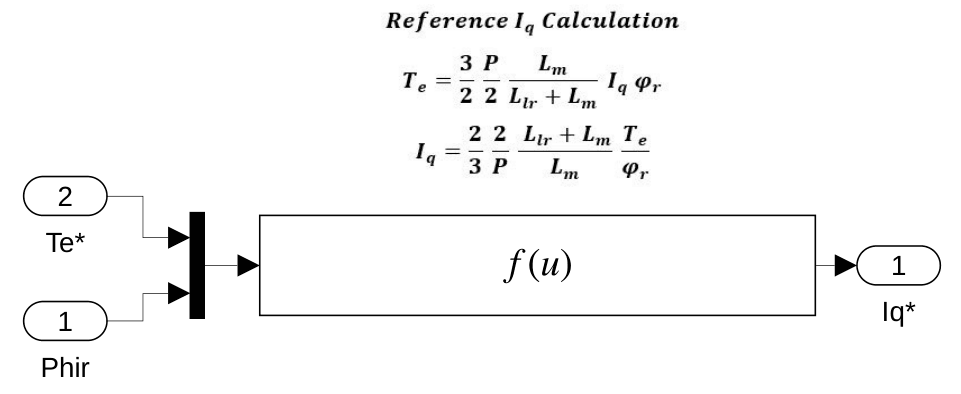
\includegraphics[width=0.9\textwidth]{VECTOR_CONTROL_FOC_OF_IM-04.png}
    \caption{Simulink Subsystem: $I_{q}^*$ Reference Calculation Block}
\end{figure}

\section{Slip and Flux Angle ($\theta_e$) Synthesis}
To maintain the required $\psi_{qr}=0$ constraint, the slip frequency ($\omega_{sl}$) is continuously calculated as:
\begin{equation}
\omega_{sl} = \frac{L_{m}}{\tau_{r}} \cdot \frac{i_{qs}^*}{\psi_{r}^*} = \frac{0.0347}{0.1557} \cdot \frac{i_{qs}^*}{0.96} = 0.2228 \cdot \frac{i_{qs}^*}{0.96} = 0.232 \cdot i_{qs}^* \text{ rad/s}
\end{equation}
The mechanical rotor speed ($\omega_m$) is scaled to electrical speed ($\omega_r = \omega_m \frac{P}{2} = 2\omega_m$). The synchronous speed is:
\begin{equation}
\omega_{e} = \omega_{r} + \omega_{sl} = 2\omega_{m} + 0.232 \cdot i_{qs}^* \text{ rad/s}
\end{equation}
The flux angle ($\theta_e$) is then calculated through discrete numerical integration (Forward Euler) wrapped inside a modulo $2\pi$ function to avoid DSP register overflow during high-speed rotation:
\begin{equation}
\theta_{e}[k] = (\theta_{e}[k-1] + \omega_{e}[k] \cdot T_{s}) \pmod{2\pi}
\end{equation}

\begin{figure}[H]
    \centering
    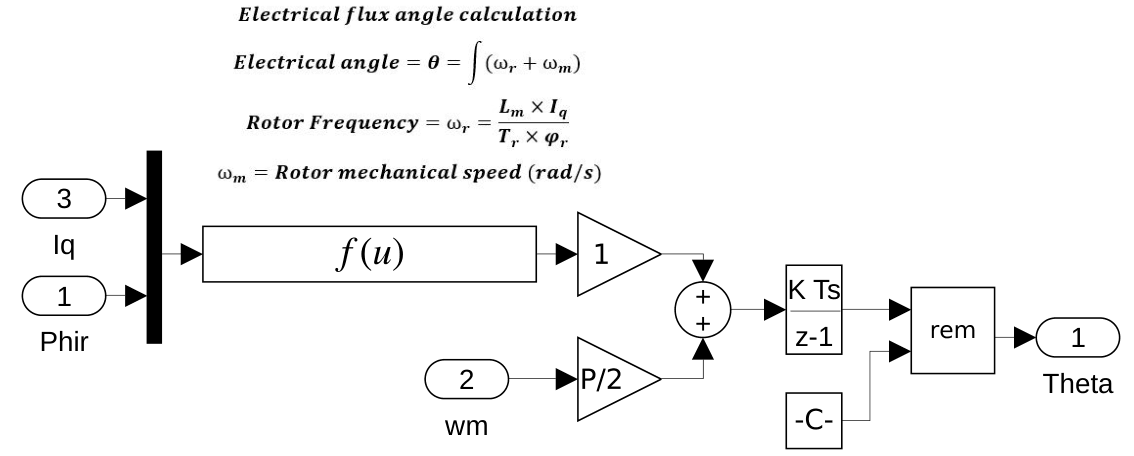
\includegraphics[width=0.8\textwidth]{VECTOR_CONTROL_FOC_OF_IM-05.png}
    \caption{Simulink Subsystem: IFOC Slip and Flux Angle Estimation}
\end{figure}
\begin{figure}[H]
    \centering
    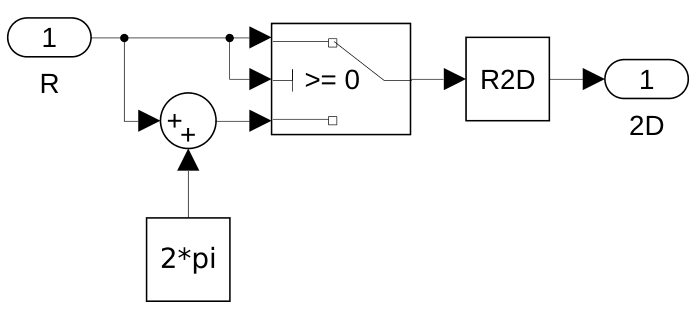
\includegraphics[width=0.8\textwidth]{VECTOR_CONTROL_FOC_OF_IM-15.png}
    \caption{Simulink Subsystem: Modulo $2\pi$ Restraint Loop}
\end{figure}

\begin{figure}[H]
    \centering
    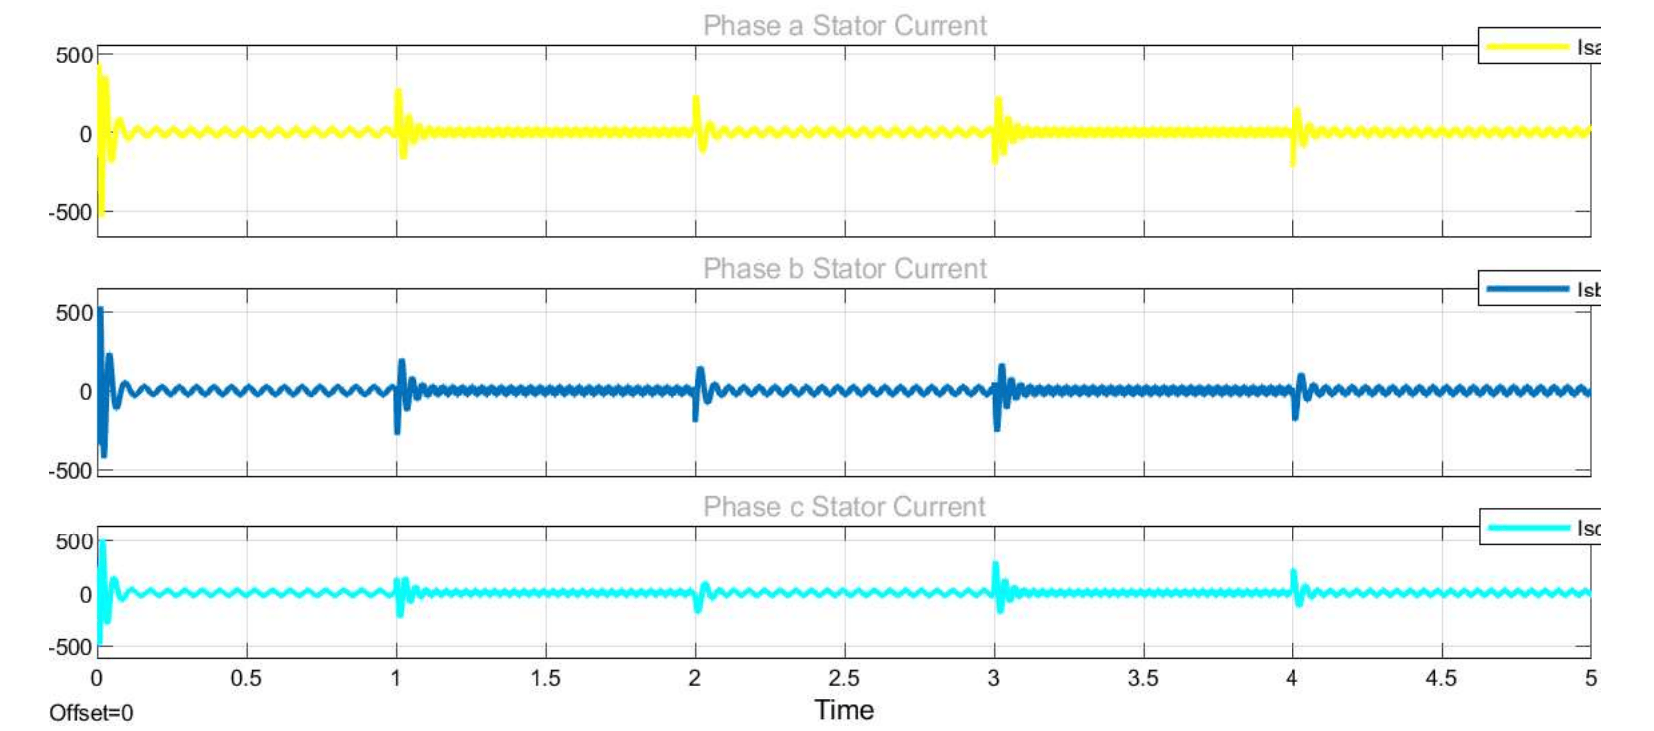
\includegraphics[width=0.9\textwidth]{23.png}
    \caption{Scope Output: Three-Phase Stator Currents Responding to Load Transients}
\end{figure}


\chapter{Space Vector Pulse Width Modulation (SVPWM)}
\section{SVPWM Overview}
The final control actuation is executed by a Three-Phase Voltage Source Inverter using Space Vector Pulse Width Modulation (SVPWM). SVPWM treats the inverter as a single, cohesive unit capable of producing eight discrete voltage vectors. It enhances DC bus utilisation by up to 15.47\% over standard SPWM and significantly minimizes Total Harmonic Distortion (THD).

\begin{figure}[H]
    \centering
    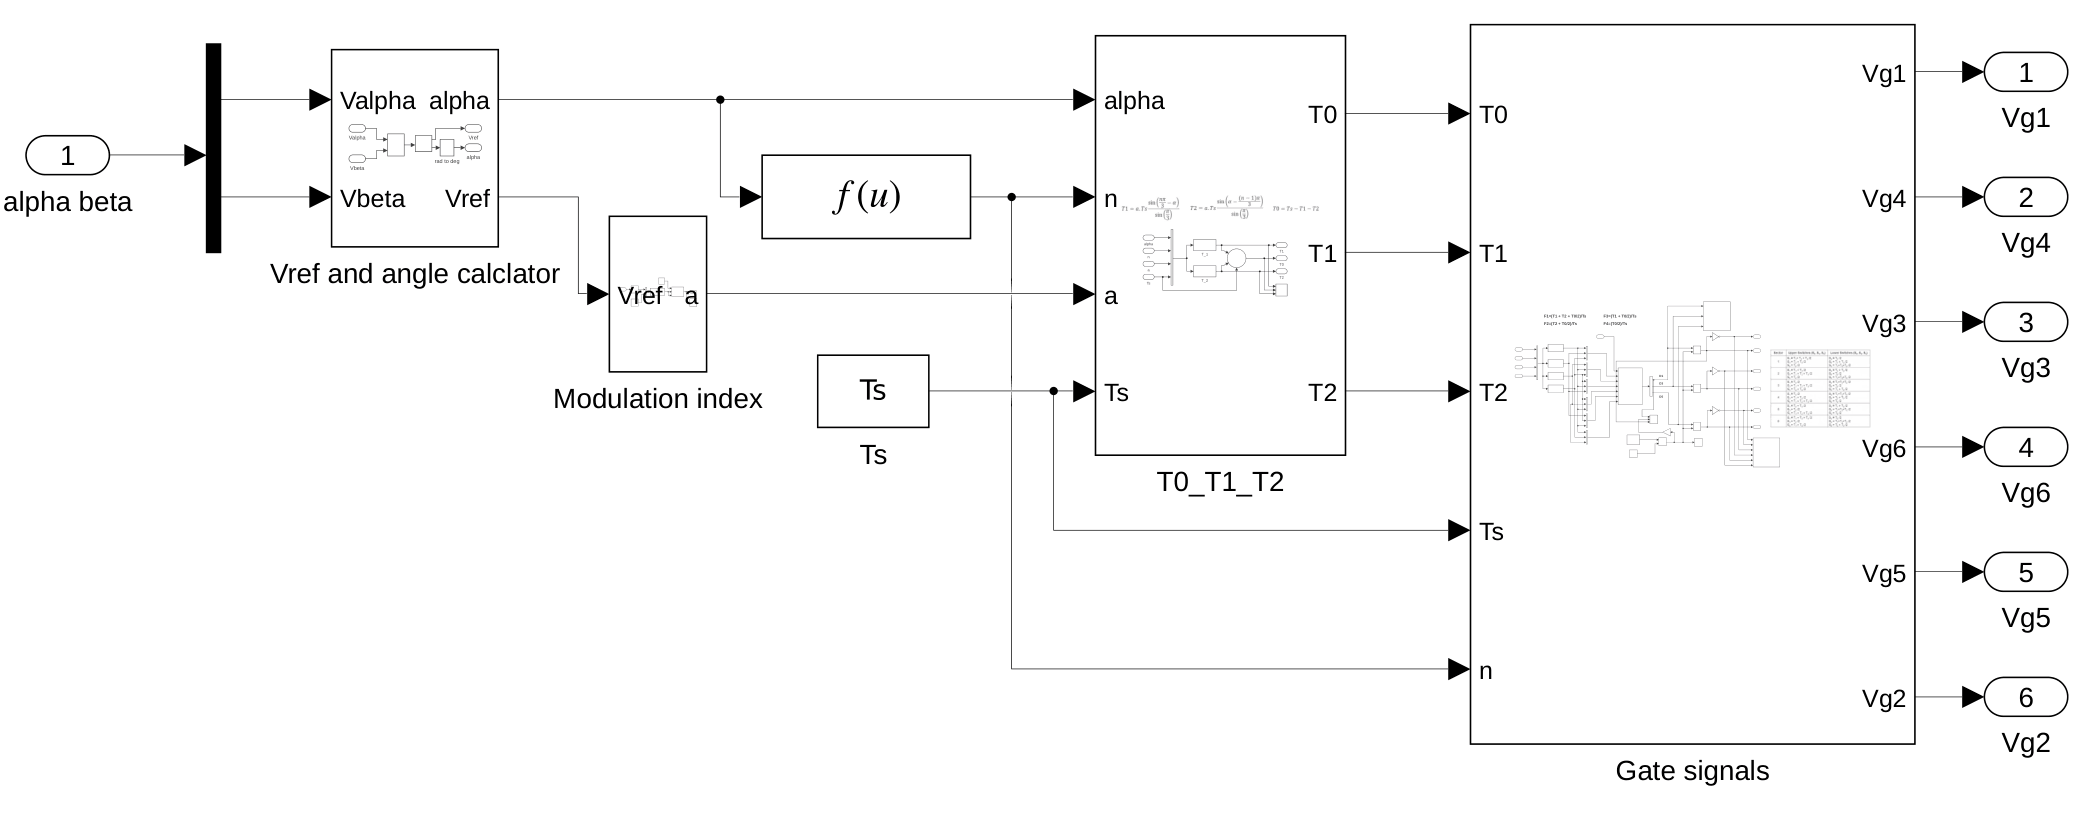
\includegraphics[width=1.0\textwidth]{VECTOR_CONTROL_FOC_OF_IM-10.png}
    \caption{Main Architecture of the Space Vector PWM Generation Subsystem}
\end{figure}

\section{Reference Vector Synthesis and Dwell Times}
The stationary frame commands, $v_{\alpha}^*$ and $v_{\beta}^*$, form the reference vector $\vec{V}_{ref}$. 
\begin{align}
|\vec{V}_{ref}| &= \sqrt{(v_{\alpha}^*)^2 + (v_{\beta}^*)^2} \\
\theta_{ref} &= \arctan\left(\frac{v_{\beta}^*}{v_{\alpha}^*}\right)
\end{align}
For example, if the current control loop commands $v_{\alpha}^* = 300$ V and $v_{\beta}^* = 400$ V:
\begin{align}
|\vec{V}_{ref}| &= \sqrt{(300)^2 + (400)^2} = \sqrt{250000} = 500 \text{ V} \\
\theta_{ref} &= \arctan\left(\frac{400}{300}\right) = 53.13^\circ
\end{align}
This locates the reference vector inside Sector 1.

\begin{figure}[H]
    \centering
    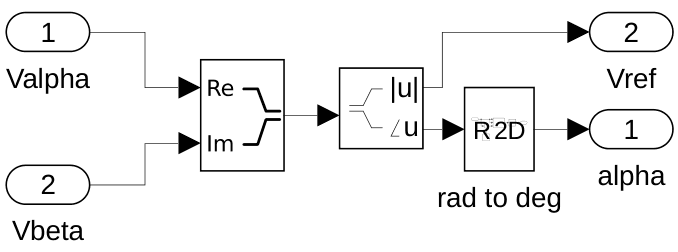
\includegraphics[width=0.8\textwidth]{VECTOR_CONTROL_FOC_OF_IM-14.png}
    \caption{Simulink Subsystem: Transformation to Magnitude and Angle}
\end{figure}

\begin{figure}[H]
    \centering
    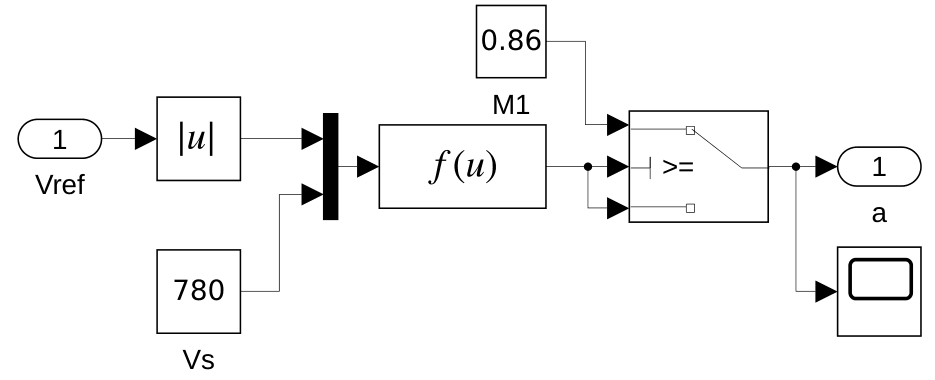
\includegraphics[width=0.8\textwidth]{VECTOR_CONTROL_FOC_OF_IM-12.png}
    \caption{Simulink Subsystem: Modulation Index and Overmodulation Safeguard}
\end{figure}

The dwell times ($T_1, T_2$) for the active adjacent vectors are evaluated over switching period $T_s = 2 \mu s$ utilizing volt-second balancing:
\begin{align}
T_{1} &= \frac{\sqrt{3} \cdot T_{s} \cdot |\vec{V}_{ref}|}{V_{dc}} \sin\left(\frac{\pi}{3} - \theta^{\prime}\right) \\
T_{2} &= \frac{\sqrt{3} \cdot T_{s} \cdot |\vec{V}_{ref}|}{V_{dc}} \sin(\theta^{\prime}) \\
T_{0} &= T_{s} - T_{1} - T_{2}
\end{align}
Using $V_{dc} = 780$ V and $|\vec{V}_{ref}| = 500$ V at $\theta^{\prime} = 53.13^\circ$:
\begin{align}
\text{Factor} &= \frac{\sqrt{3} \times (2 \times 10^{-6}) \times 500}{780} = 2.22 \times 10^{-6} \text{ s} \\
T_{1} &= 2.22 \times 10^{-6} \cdot \sin(60^\circ - 53.13^\circ) = 2.22 \mu\text{s} \times 0.119 = 0.265 \mu\text{s} \\
T_{2} &= 2.22 \times 10^{-6} \cdot \sin(53.13^\circ) = 2.22 \mu\text{s} \times 0.8 = 1.776 \mu\text{s} \\
T_{0} &= 2.0 - 0.265 - 1.776 = -0.041 \mu\text{s} \rightarrow 0 \mu\text{s} \text{ (Saturated)}
\end{align}

\begin{figure}[H]
    \centering
    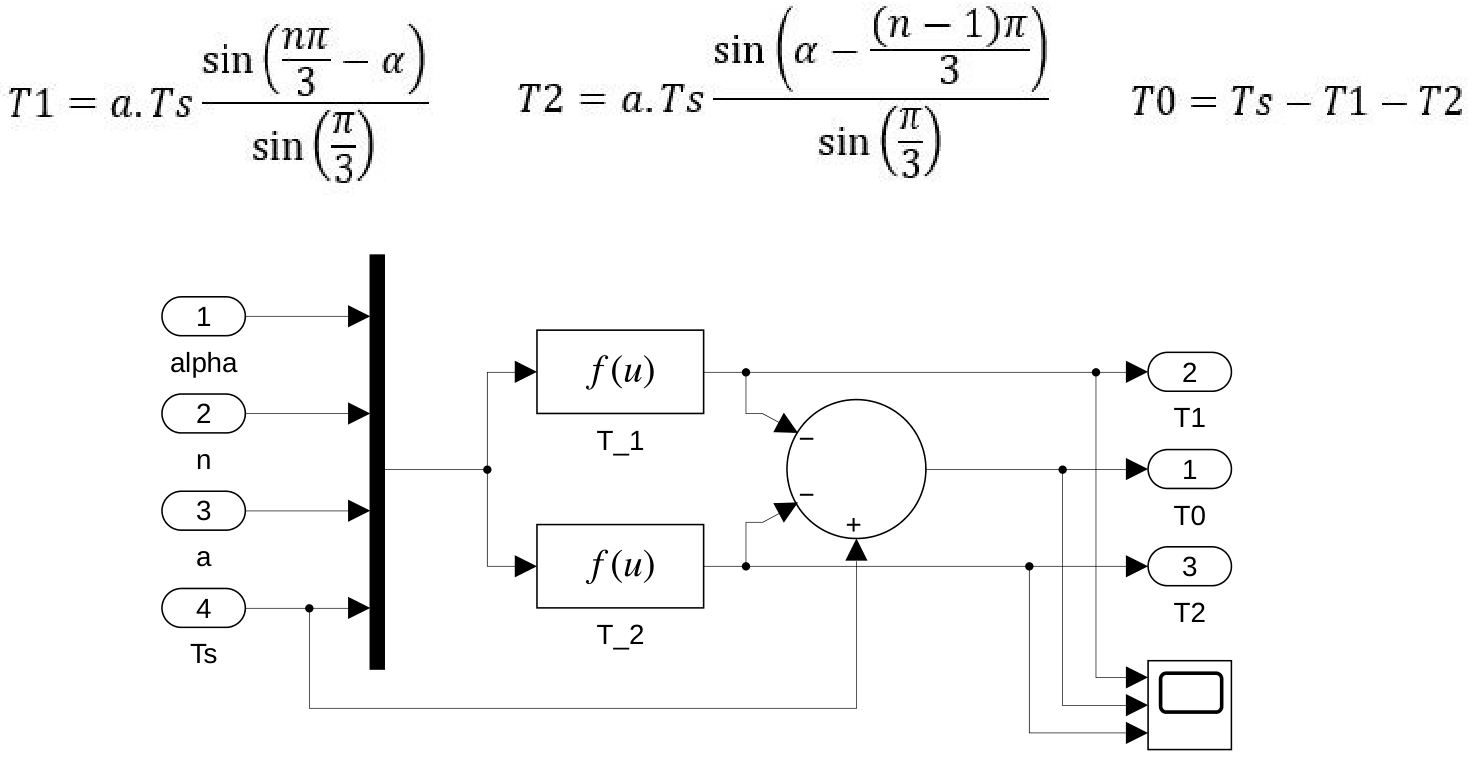
\includegraphics[width=0.9\textwidth]{VECTOR_CONTROL_FOC_OF_IM-13.png}
    \caption{Simulink Subsystem: Dwell Time Calculation based on Sector and Angle}
\end{figure}
\begin{figure}[H]
    \centering
    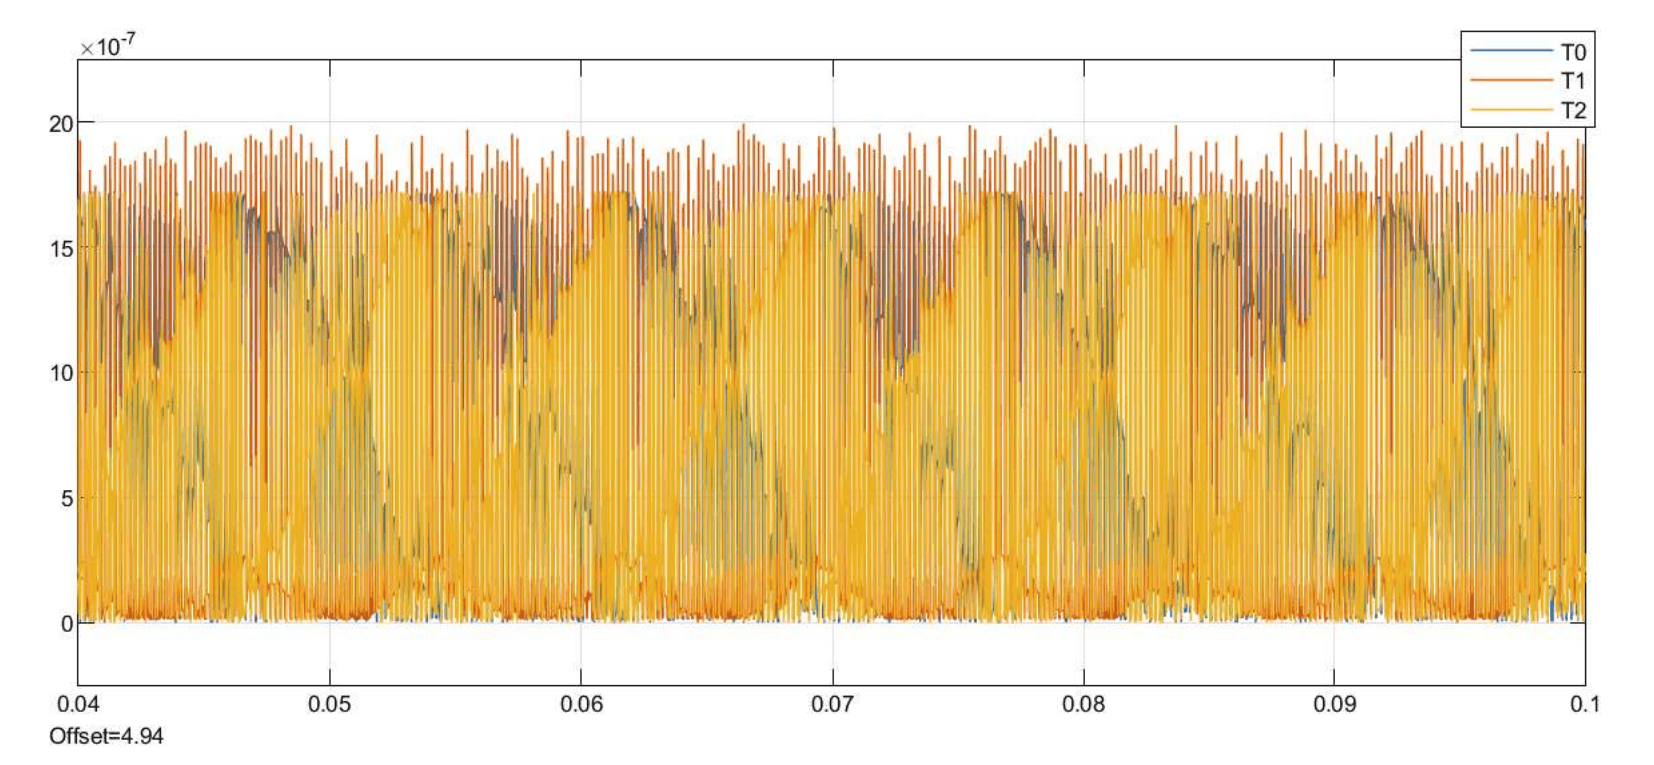
\includegraphics[width=0.9\textwidth]{31.png}
    \caption{Scope Output: Calculated Dwell Times across Switching Periods}
\end{figure}

\section{Switching Logic and Gate Sequences}
\begin{figure}[H]
    \centering
    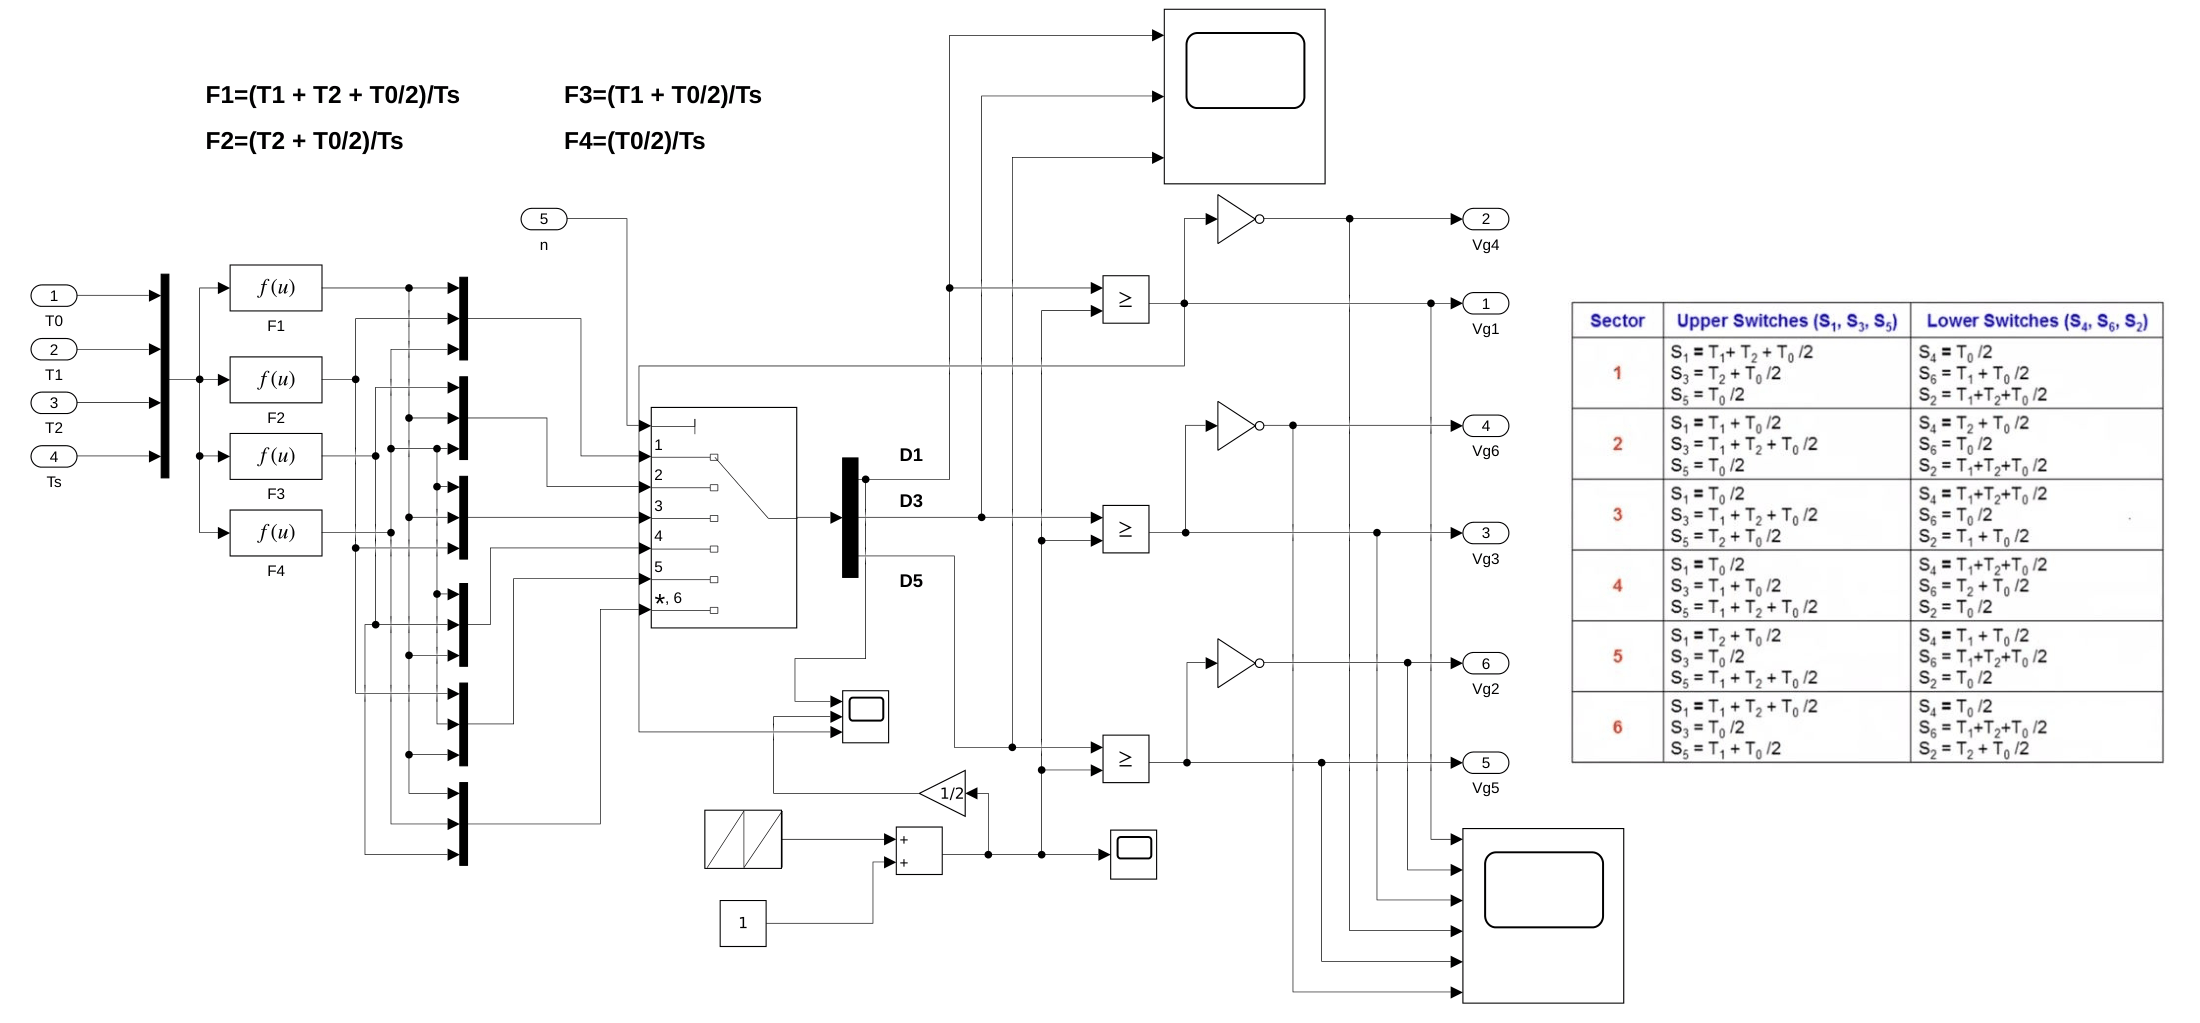
\includegraphics[width=1.0\textwidth]{VECTOR_CONTROL_FOC_OF_IM-11.png}
    \caption{Simulink Subsystem: Detailed PWM Logic and Gate Signal Routing}
\end{figure}
\begin{figure}[H]
    \centering
    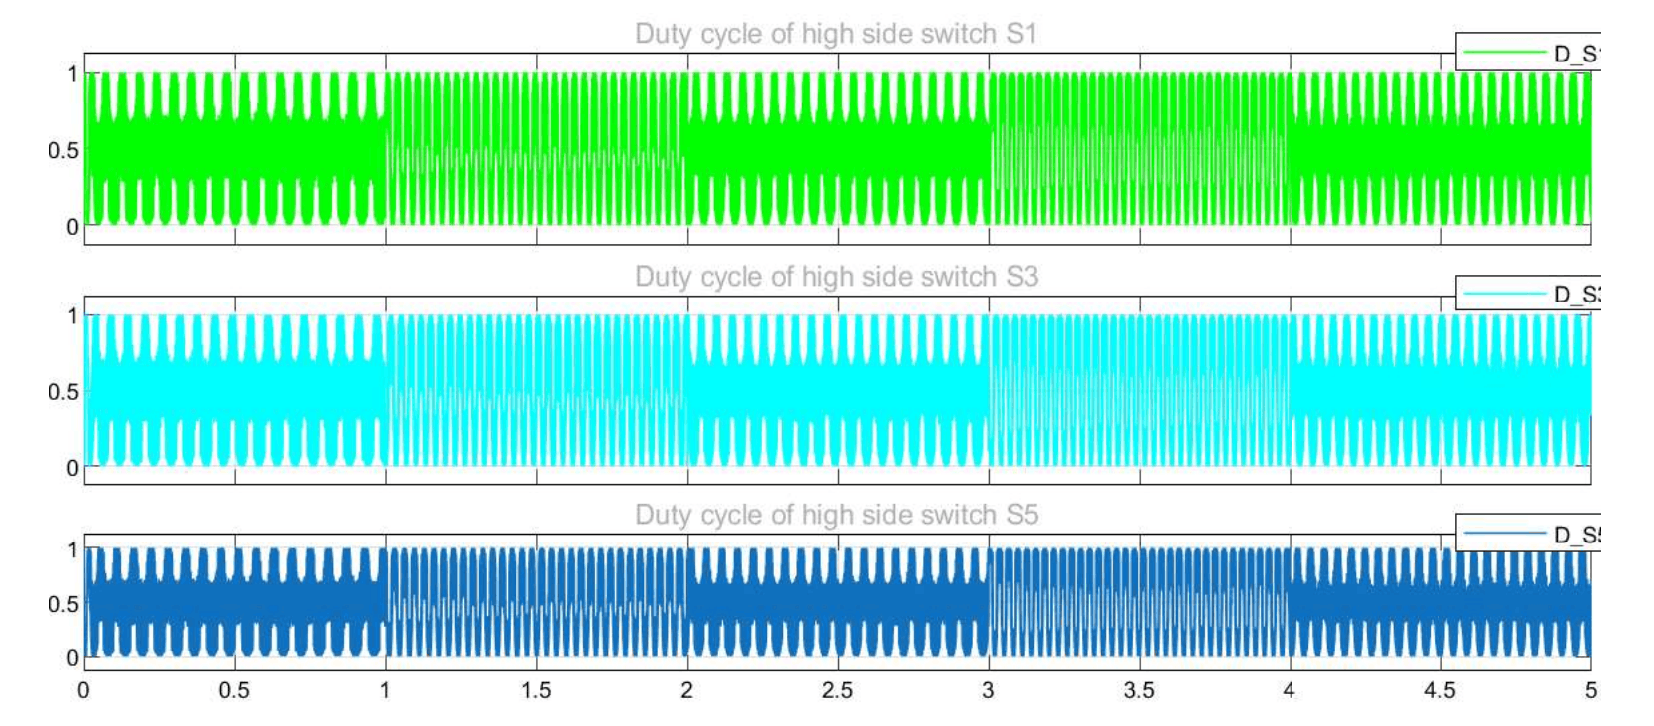
\includegraphics[width=0.9\textwidth]{32.png}
    \caption{Scope Output: Duty Cycles of High-Side Switches across Sectors}
\end{figure}
\begin{figure}[H]
    \centering
    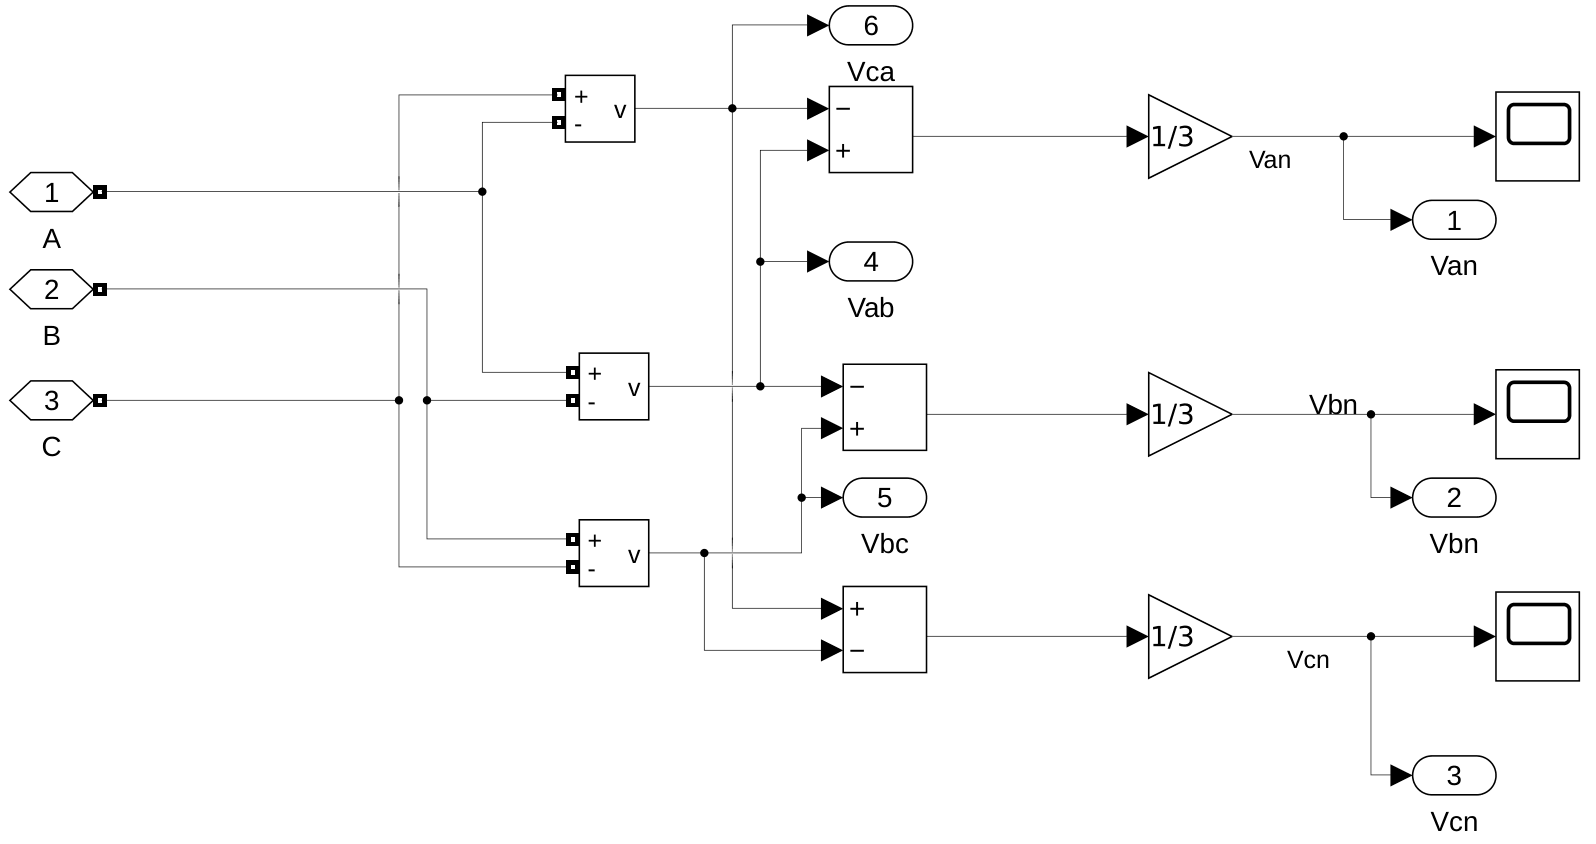
\includegraphics[width=0.9\textwidth]{VECTOR_CONTROL_FOC_OF_IM-08.png}
    \caption{Simulink Subsystem: Three-Phase and Line-to-Line Voltage Processing}
\end{figure}


\chapter{Conclusion and Future Scope}
\section{Conclusions}
The provided Simulink model serves as far more than a mere theoretical exercise; it is a highly accurate, functionally complete "digital twin" of a modern, industrial-grade Indirect Field Oriented Control (IFOC) system for a 50 HP Squirrel-Cage Induction Motor. By meticulously modelling the electromechanical plant, the coordinate transformations, and the discrete-time control logic, this architecture successfully demystifies the complex, non-linear dynamics inherent in three-phase AC machines.

By projecting the stator currents into a synchronously rotating $d-q$ reference frame, the architecture proves that an induction motor can be controlled with the same orthogonal precision and dynamic transient response as a separately excited DC motor. The simulation successfully bridges the critical gap between continuous-time control theory and practical digital implementation executing at a strict $2\mu s$ sample time.

\section{Future Scope}
Future enhancements to this model can include sensorless IFOC through advanced state observers (such as Model Reference Adaptive Systems or Extended Kalman Filters) to eliminate the requirement for a physical mechanical speed encoder. Furthermore, the incorporation of thermal detuning adaptation algorithms to adjust the rotor time constant $R_r$ dynamically will vastly improve torque-tracking stability under high-temperature operating conditions.

\begin{thebibliography}{9}
\bibitem{foc_paper}
"Comprehensive Analysis of Field Oriented Control (FOC) for a 3-Phase Induction Motor", Professor of Electrical Engineering, June 12, 2026.
\end{thebibliography}

\end{document}